%%%%%%%% ICML 2023 EXAMPLE LATEX SUBMISSION FILE %%%%%%%%%%%%%%%%%

\documentclass{article}

% Recommended, but optional, packages for figures and better typesetting:
\usepackage{microtype}
\usepackage{graphicx}
\usepackage{subfigure}
\usepackage{booktabs} % for professional tables

\usepackage{tikz}
% Corporate Design of the University of Tübingen
% Primary Colors
\definecolor{TUred}{RGB}{165,30,55}
\definecolor{TUgold}{RGB}{180,160,105}
\definecolor{TUdark}{RGB}{50,65,75}
\definecolor{TUgray}{RGB}{175,179,183}

% Secondary Colors
\definecolor{TUdarkblue}{RGB}{65,90,140}
\definecolor{TUblue}{RGB}{0,105,170}
\definecolor{TUlightblue}{RGB}{80,170,200}
\definecolor{TUlightgreen}{RGB}{130,185,160}
\definecolor{TUgreen}{RGB}{125,165,75}
\definecolor{TUdarkgreen}{RGB}{50,110,30}
\definecolor{TUocre}{RGB}{200,80,60}
\definecolor{TUviolet}{RGB}{175,110,150}
\definecolor{TUmauve}{RGB}{180,160,150}
\definecolor{TUbeige}{RGB}{215,180,105}
\definecolor{TUorange}{RGB}{210,150,0}
\definecolor{TUbrown}{RGB}{145,105,70}

% hyperref makes hyperlinks in the resulting PDF.
% If your build breaks (sometimes temporarily if a hyperlink spans a page)
% please comment out the following usepackage line and replace
% \usepackage{icml2023} with \usepackage[nohyperref]{icml2023} above.
\usepackage{hyperref}


% Attempt to make hyperref and algorithmic work together better:
\newcommand{\theHalgorithm}{\arabic{algorithm}}

\usepackage[accepted]{icml2023}

% For theorems and such
\usepackage{amsmath}
\usepackage{amssymb}
\usepackage{mathtools}
\usepackage{amsthm}

% if you use cleveref..
\usepackage[capitalize,noabbrev]{cleveref}

%%%%%%%%%%%%%%%%%%%%%%%%%%%%%%%%
% THEOREMS
%%%%%%%%%%%%%%%%%%%%%%%%%%%%%%%%
\theoremstyle{plain}
\newtheorem{theorem}{Theorem}[section]
\newtheorem{proposition}[theorem]{Proposition}
\newtheorem{lemma}[theorem]{Lemma}
\newtheorem{corollary}[theorem]{Corollary}
\theoremstyle{definition}
\newtheorem{definition}[theorem]{Definition}
\newtheorem{assumption}[theorem]{Assumption}
\theoremstyle{remark}
\newtheorem{remark}[theorem]{Remark}

% Todonotes is useful during development; simply uncomment the next line
%    and comment out the line below the next line to turn off comments
%\usepackage[disable,textsize=tiny]{todonotes}
\usepackage[textsize=tiny]{todonotes}


% The \icmltitle you define below is probably too long as a header.
% Therefore, a short form for the running title is supplied here:
\icmltitlerunning{Project Report Template for Data Literacy 2023/24}

\begin{document}

\twocolumn[
\icmltitle{Are You Still Booking Train Tickets Under the Assumption of \\ No Delays?}

% It is OKAY to include author information, even for blind
% submissions: the style file will automatically remove it for you
% unless you've provided the [accepted] option to the icml2023
% package.

% List of affiliations: The first argument should be a (short)
% identifier you will use later to specify author affiliations
% Academic affiliations should list Department, University, City, Region, Country
% Industry affiliations should list Company, City, Region, Country

% You can specify symbols, otherwise they are numbered in order.
% Ideally, you should not use this facility. Affiliations will be numbered
% in order of appearance and this is the preferred way.
\icmlsetsymbol{equal}{*}

\begin{icmlauthorlist}
\icmlauthor{Sumitrra Bala Subramaniam}{equal,first}
\icmlauthor{Jiha Kim}{equal,second}
\icmlauthor{Frederik Panse}{equal,third}
\icmlauthor{Kim Isabella Zierahn}{equal,fourth}
\end{icmlauthorlist}

% fill in your matrikelnummer, email address, degree, for each group member
\icmlaffiliation{first}{Matrikelnummer 6642271, sumitrra.bala-subramaniam@student.uni-tuebingen.de, MSc Quantitative Data Science Methods}
\icmlaffiliation{second}{Matrikelnummer 6640082, jiha.kim@student.uni-tuebingen.de, MSc Quantitative Data Science Methods}
\icmlaffiliation{third}{Matrikelnummer 5810899, frederik.panse@student.uni-tuebingen.de, MSc Quantitative Data Science Methods}
\icmlaffiliation{fourth}{Matrikelnummer 6635183, kim-isabella.zierahn@student.uni-tuebingen.de, MSc Quantitative Data Science Methods}

% You may provide any keywords that you
% find helpful for describing your paper; these are used to populate
% the "keywords" metadata in the PDF but will not be shown in the document
\icmlkeywords{Machine Learning, ICML}

\vskip 0.3in
]

% this must go after the closing bracket ] following \twocolumn[ ...

% This command actually creates the footnote in the first column
% listing the affiliations and the copyright notice.
% The command takes one argument, which is text to display at the start of the footnote.
% The \icmlEqualContribution command is standard text for equal contribution.
% Remove it (just {}) if you do not need this facility.

%\printAffiliationsAndNotice{}  % leave blank if no need to mention equal contribution
\printAffiliationsAndNotice{\icmlEqualContribution} % otherwise use the standard text.

\begin{abstract}
In 2022, Deutsche Bahn reported that one in three of its trains was late, underscoring the importance of finding the most reliable route, not just the fastest. We conduct route optimization to find the most reliable route going from Stuttgart to Frankfurt (Main), analyze factors that influence the train delays, and create a Random Forest model, using data provided by Deutsche Bahn. The optimal route has less than half of the mean delay of the fastest route that Deutsche Bahn offers. The train delay is most influenced by the route's proximity to the German border, the (relative) number of train rides and the betweenness centrality. This project highlights the fact that opting for the minimum time is not always the best choice.
\end{abstract}

\section{Introduction}\label{sec:intro}
If a group of students from Tübingen wants to take a train trip to Frankfurt (Main), there are many potential routes they could take. Would they be able to decide beforehand on the most reliable route and the best time to go?

People determine their train schedules under the assumption of no train delays. However, when Deutsche Bahn announced that its \href{https://zbir.deutschebahn.com/2023/en/interim-group-management-report-unaudited/product-quality-and-digitalization/punctuality/}{punctuality quote} fell to 65.2 percent in 2022, this assumption has become problematic. When traveling from one place to another via Deutsche Bahn, passengers often can't rely on arriving at their destination at the scheduled time. Although Deutsche Bahn provides real-time information on train delays, passengers are not informed beforehand of likely delays. Deutsche Bahn is able to identify the fastest route, without considering the mean delay of this route (e.g., \href{https://www.bahn.de/buchung/intern/start}{travel information}). Previous studies often focused on predicting train delay \cite{predtraindelay, largetrainnet, MLtraindel}. Our goal is to identify the most reliable train route going from Stuttgart to Frankfurt (Main).

To analyze the most reliable route, we are following two approaches: route optimization (\Cref{sec:methods_route}) and analysing external influences (\Cref{sec:methods_ext}). The first approach is to find all possible routes going from Stuttgart to Frankfurt (Main) and then identifying the route with the least mean delay (i.e., the most reliable route). Our results show that the optimal route differs from the fastest route that Deutsche Bahn offers (\Cref{sec:results_route}). The second approach is to investigate whether e.g., the day of the week, holidays, the station's distance to the border or number of trains per station impact the delay. Our findings display several factors influencing the delay (\Cref{sec:results_ext}).

We shed further light on one factor: weekdays versus weekends. Regular passengers often use the train either to commute to work on weekdays or to get home on weekends, so it is important to consider the day of travel when choosing a route. As this information is relevant to end-consumers, we analyze whether the overall most reliable route is also optimal when considering only weekdays or weekends.

We aim to fill a gap in train delay research by shifting the focus from predicting delays to providing passengers with pre-trip information on the most reliable route and the best time to travel. This allows passengers to make informed decisions about their travel, allowing them to choose the optimal route with confidence, rather than relying solely on the fastest route.


\section{Data and Methods}\label{sec:methods}

We use \href{https://data.deutschebahn.com/dataset/ist-verkehrsdaten-der-db-cargo-auf-bst8-ebene.html}{train delay data} provided by Deutsche Bahn (DB) which consists of stations and stops that measured the number of trains and minutes of delay of all trains passing by in 2016. We are also using the \href{https://data.deutschebahn.com/dataset/betriebsstellen-gueterverkehr.html}{directory of operating sites}, containing the names and coordinates of the stations. For geographical information on routes of the rail network, we use \href{https://data.deutschebahn.com/dataset/betriebsstellen-gueterverkehr.html}{geographical route data}. Our train delay data consists of 757 007 entries, measuring the delay all over Germany throughout the year 2016. Figure~\ref{all_data_cmap} shows an overview of all stops and stations and their mean delay in 2016. The mean delay of all stations in Germany in 2016 was 34.84 minutes. After merging all three datasets, our data consists of information about the stations and stops, their time stamp, their geographical data, their corresponding nearest routes and further information about the rails (e.g., railroad type, number of rails, speed limit or electrification). All analyses are conducted in Python \cite{1995python}.

\begin{figure} % this figure made with
% plt.rcParams.update(bundles.icml2022(column=”half”, nrows=num_rows, ncols=num_cols, usetex=False)))
% fig,ax = plt.subplots(nrows=num_rows, ncols=num_cols)
\begin{center}
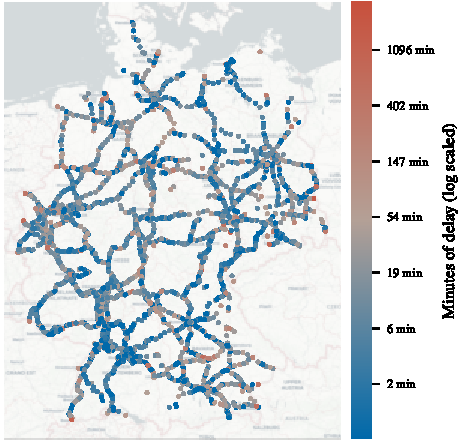
\includegraphics{./fig/maps_KI_01_all_data_cmap.pdf} % note no [width=\textwidth] needed
\end{center}
\caption{Mean delay of trains in 2016 for all available stations in Germany. Map data © \href{https://www.openstreetmap.org/}{OpenStreetMap} contributors © CARTO.}
\label{all_data_cmap}
\end{figure}

\subsection{Route Optimization}\label{sec:methods_route}

Our first approach is to find the optimal route from Stuttgart to Frankfurt (Main) (i.e., the route with the least mean delay). Using the geographical route data, we first get all continuous routes that exist in Germany. Then, all routes starting in Stuttgart are identified. From here, we identify all adjacent routes that connect to these starting routes. We repeatedly find adjacent routes until all possible routes are collected, starting in Stuttgart and terminating in Frankfurt (Main). Next, the route data is connected to the stations that measured the delay (i.e., the mean delay data). This is conducted by assigning the stations to the route to which it has a distance that is less or equal to 0.01 latitudes and longitudes. This translates to a maximum distance to the matching route of about 0.7 to 1.11 km, depending on the specific latitude or longitude. Finally, the mean delay is calculated for each possible route and the route with the lowest mean delay is determined.

To compare our optimal route with the fastest route offered by DB, we took the fastest route and its schedule from the DB website. We manually collect all the stations along the fastest route and calculate the mean delay for this route.


\subsection{Factors Influencing Delays}\label{sec:methods_ext}

The second approach is to identify factors that influence the delay.  Several features are analyzed, including characteristics of the day (e.g., weekday, month, whether it is a holiday), characteristics of the station (e.g., the number of train rides at a station, the station's distance to the border) and centrality measures. We conduct a Random Forest model to examine which factors influence the train delay the most. It provides information about factors influencing the delay and their importance. According to \citet{rogers2006identifying}, due to the random exploration of features, Random Forest lends itself to feature selection well and the measure of feature importance adopted here is the average information gain achieved during forest construction.

To determine if there is a more reliable route than the overall optimal one based on whether you are traveling on a weekday or weekend, we calculate the mean delay for each possible path on weekdays and weekends in addition to the overall mean. We then compare them visually.

\subsubsection{Centrality Measures}

Centrality measures demonstrate the level of interaction between stations, indicating how connected a station is to other stations. Betweenness centrality is a crucial indicator for a node (i.e., a train station) because it refers to how central it is for being between other stations \cite{betweenness}. It is crucial for the transportation of passengers \cite{centrality} and measures the extent to which a station serves as a connection between other stations.

For a better understanding of the relationship between stations, we calculate the correlation between stations and only considered correlations that are 0.4 or higher. Then we calculate the centrality measures. Betweenness centrality for a station is calculated by counting how many times that station is part of the shortest paths between other stations. The more often it acts as a bridge or connector in the network, the higher its betweenness centrality \cite{centrality}.

The second centrality measure is closeness centrality. Closeness centrality for a station is a measure of how quickly it can reach all other stations in the network. If a station has high closeness centrality, it's relatively close to many other stations, indicating efficient communication or transportation within the network \cite{generic_comp}.

% This is the template for a figure from the original ICML submission pack. In lecture 10 we will discuss plotting in detail.
% Refer to this lecture on how to include figures in this text.
%
% \begin{figure}[ht]
% \vskip 0.2in
% \begin{center}
% \centerline{\includegraphics[width=\columnwidth]{icml_numpapers}}
% \caption{Historical locations and number of accepted papers for International
% Machine Learning Conferences (ICML 1993 -- ICML 2008) and International
% Workshops on Machine Learning (ML 1988 -- ML 1992). At the time this figure was
% produced, the number of accepted papers for ICML 2008 was unknown and instead
% estimated.}
% \label{icml-historical}
% \end{center}
% \vskip -0.2in
% \end{figure}

\section{Results}\label{sec:results}

\subsection{Route Optimization}\label{sec:results_route}

There are 54 unique routes, all starting in Stuttgart and ending in Frankfurt (Main). We found the optimal route with the least mean delay, including 42 stations or stops. The mean delay for our optimal route is 14.19 minutes. The fastest route offered by DB contains 46 stations or stops with a mean delay of 35.65 minutes. Figure~\ref{rel_fast_zoomed} displays a comparison of both routes.\footnote{More visualizations and the code can be found on our \href{https://github.com/frederikpanse/db_project}{github repository}.} Both routes start in a similar direction, via Vaihingen to Mannheim. They continue in two different directions. Our optimal route is via Worms, Mainz and Frankfurt Airport, while the fastest DB route is via Weinheim, Bensheim and Darmstadt to Frankfurt (Main).

\begin{figure} % this figure made with
% plt.rcParams.update(bundles.icml2022(column=”half”, nrows=num_rows, ncols=num_cols, usetex=False)))
% fig,ax = plt.subplots(nrows=num_rows, ncols=num_cols)
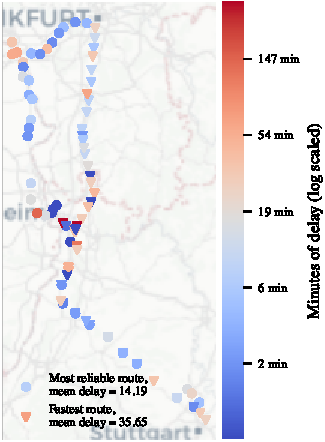
\includegraphics{./fig/maps_KI_03_reliable_vs_fastest_zoomed_Carto.pdf} % note no [width=\textwidth] needed
\caption{Most reliable route by our analyses and fastest route that Deutsche Bahn offers. Map data © \href{https://www.openstreetmap.org/}{OpenStreetMap} contributors © CARTO.}
\label{rel_fast_zoomed}
\end{figure}

\subsection{Factors Influencing Delays}\label{sec:results_ext}

The dataset we use in this study is characterized by a significant imbalance, with a large proportion of non-delayed data. To tackle this, we apply downsampling, focusing on the count of delayed instances. The accuracy of the Random Forest model is 0.8229. Figure~\ref{feature_importance} gives an overview of all features and their importance for the delay.


\begin{figure}
    \centering
    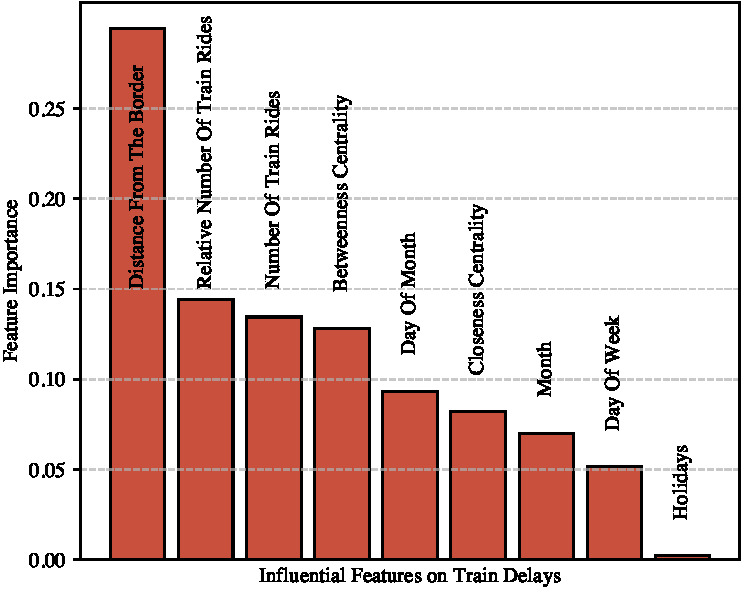
\includegraphics[width=1\linewidth]{./fig/plot_JH_01_feature_importance.pdf}
    \caption{Feature Importance of Random Forest}
    \label{feature_importance}
\end{figure}

\subsubsection{Characteristics of the day}

Of all the factors we analyzed, the characteristics of the day,  such as the weekday, month, or whether it is a holiday, have the least influence on the delay (Figure~\ref{feature_importance}). 

As shown in Figure~\ref{we_wd}, the overall most reliable route is also the most reliable route when only considering weekdays or weekends. The overall 7th most reliable route, however, has only about 3 seconds more mean delay on weekends than the the most reliable route. Figure~\ref{we_wd} also reveals the systematic pattern that weekend travelling is more reliable than on weekdays. Trains have about 19 minutes less delay on weekends than on weekdays.

\begin{figure}[h]
    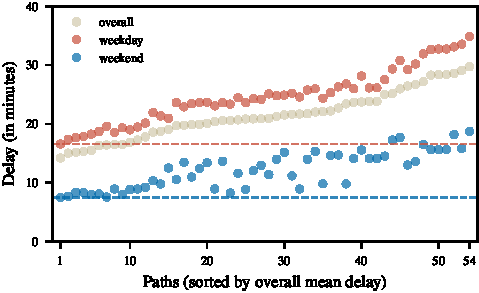
\includegraphics{./fig/plot_FP_03_WeekdayWeekend.pdf}
    \caption{Comparing weekday and weekend mean delay for each route. The red and blue dashed lines show the mean delay for the most reliable route on weekdays and weekends, respectively.}
    \label{we_wd}
\end{figure}

\subsubsection{Characteristics of the station}

We consider three factors related to train stations, listed in order of variable importance: distance from the border, the ratio of the given date's train rides to the median of the usual train rides (relative number of train rides), and the number of train rides. 

\subsubsection{Centrality Measures}

As seen in Figure~\ref{feature_importance}, the betweenness centrality can serve as a very useful tool to plan their schedule because the more ‘central’ stations experience much more stress, resulting in high delays \cite{centrality}. 


\section{Discussion \& Conclusion}\label{sec:conclusion}

The aim of our study is to find the most reliable route from Stuttgart to Frankfurt (Main). To do so, we conduct route optimization and propose an optimized route that has less than half of the mean delay than the fastest route proposed by DB. In addition to that, we analyze external factors that might influence train delay and find that the route's distance to the border of Germany, the (relative) number of train rides and the betweenness centrality influence train delay the most. Thus, the relative number of train rides is more significant than the absolute number. Each station has a capacity to manage operations, and if this capacity is exceeded, it will have a more substantial impact on delays than a simple increase in the number of trains.

We show that it is necessary to consider factors beyond simple travel time, such as the operational schedules of other trains and the centrality of specific stations depending on date train system. Additionally, DB operators might want to consider these factors when deciding train routes and schedules. Centrality metrics and capacity of train stations can be applied to train systems. 

We consider data from 2016, which might be outdated in 2024 and had some missing values. For example, more data was available for weekdays than for weekends, possibly influencing our results. The database used for the Random Forest model development is incomplete, incorporating only about 35.31\% of the available records. Specifically, we consider data from stations with records available for at least 288 days, accounting for over 90\% of this period. We also limit the route optimization for the route from Stuttgart to Frankfurt (Main), for now only outlining what a universal tool for finding reliable routes might look like.

The delays are computed on a daily average basis, potentially leading to varying results based on different time intervals. Furthermore, our analyses exclusively focus on delay times. A more comprehensive understanding could be achieved by constructing a model that considers both travel time and the probability of delays. 

Our results propose that there is a more reliable route than the fastest route provided by DB. This and the identification of factors influencing the train delay enables passengers to knowingly decide on the optimal route and time to go from Stuttgart to Frankfurt (Main). Our results indicate that for a trip to Frankfurt (Main), students from Tübingen should take our proposed route, preferably on the weekend, and avoid routes or stations near the border with a high number of trains passing or high betweenness centrality. 


\section*{Contribution Statement}

Sumitrra Bala Subramaniam worked on connecting the datasets and route optimization. Kim Zierahn worked on connecting the datasets and on map visualizations. Jiha Kim worked on the factors influencing the delay and the Random Forest. Frederik Panse worked on factors influencing the delay and analyzing the difference between weekdays and weekends. All authors jointly wrote the text of the report.



\bibliography{bibliography}

\bibliographystyle{icml2023}


\end{document}


% This document was modified from the file originally made available by
% Pat Langley and Andrea Danyluk for ICML-2K. This version was created
% by Iain Murray in 2018, and modified by Alexandre Bouchard in
% 2019 and 2021 and by Csaba Szepesvari, Gang Niu and Sivan Sabato in 2022.
% Modified again in 2023 by Sivan Sabato and Jonathan Scarlett.
% Previous contributors include Dan Roy, Lise Getoor and Tobias
% Scheffer, which was slightly modified from the 2010 version by
% Thorsten Joachims & Johannes Fuernkranz, slightly modified from the
% 2009 version by Kiri Wagstaff and Sam Roweis's 2008 version, which is
% slightly modified from Prasad Tadepalli's 2007 version which is a
% lightly changed version of the previous year's version by Andrew
% Moore, which was in turn edited from those of Kristian Kersting and
% Codrina Lauth. Alex Smola contributed to the algorithmic style files.
